\documentclass[tikz,border=8pt]{standalone}
% Shared look for every TikZ diagram. Load with \input{../../tools/tikz-style.tex}
\usepackage[T1]{fontenc}
\usepackage{lmodern}
\renewcommand{\sfdefault}{lmr}  % diagrams use the same serif as the text
\usetikzlibrary{arrows.meta, positioning, shapes.geometric, calc, fit, backgrounds}
\definecolor{cblue}{HTML}{4C78A8}
\definecolor{corange}{HTML}{F58518}
\definecolor{cgreen}{HTML}{54A24B}
\definecolor{cred}{HTML}{E45756}
\definecolor{cpurple}{HTML}{B279A2}
\definecolor{cgrey}{HTML}{6B6B6B}
\tikzset{
  every picture/.style={font=\sffamily, line width=1.2pt},
  box/.style={draw=#1, fill=#1!12, rounded corners=4pt, align=center, inner sep=7pt, minimum height=1.1cm},
  box/.default=cgrey,
  arrow/.style={-{Stealth[length=3mm]}, draw=cgrey, line width=1.4pt},
  title/.style={font=\sffamily\bfseries\Large},
  note/.style={font=\sffamily\small, text=cgrey, align=center},
}
\AtBeginDocument{\hyphenpenalty=10000 \exhyphenpenalty=10000}

\begin{document}
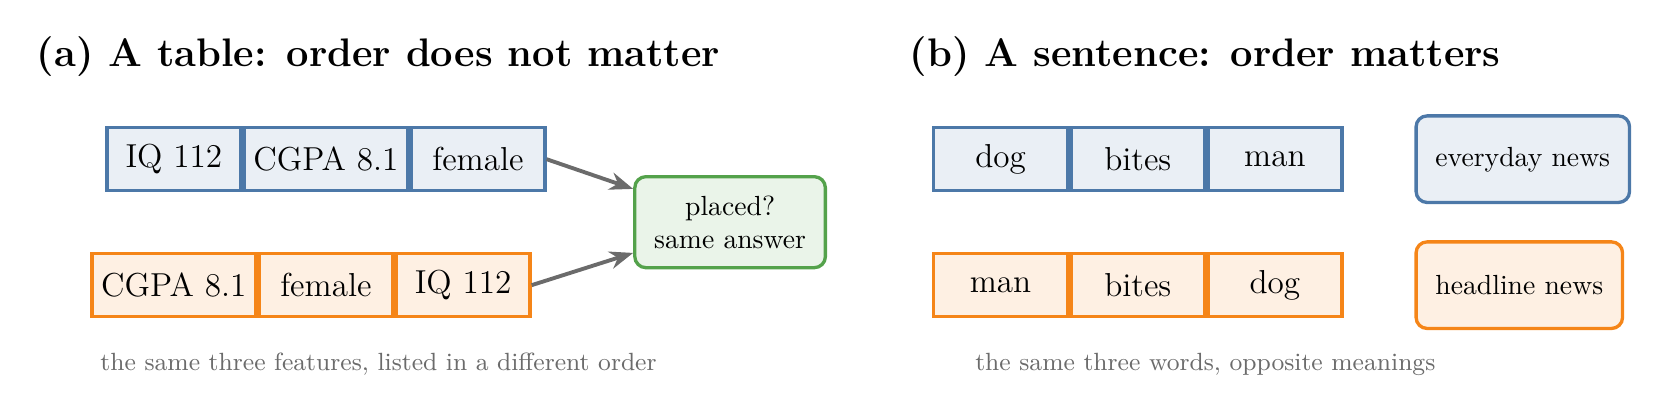
\begin{tikzpicture}[cell/.style={draw=#1, fill=#1!12, minimum width=1.7cm, minimum height=0.8cm, font=\sffamily\large}]
  % (a) tabular data: order of features does not matter
  \node[title] at (2.6, 2.3) {(a) A table: order does not matter};
  \node[cell=cblue] (a1) at (0,1) {IQ 112};
  \node[cell=cblue, right=0pt of a1] (a2) {CGPA 8.1};
  \node[cell=cblue, right=0pt of a2] (a3) {female};
  \node[cell=corange] (b1) at (0,-0.6) {CGPA 8.1};
  \node[cell=corange, right=0pt of b1] (b2) {female};
  \node[cell=corange, right=0pt of b2] (b3) {IQ 112};
  \node[box=cgreen, right=1.1cm of a3, yshift=-0.8cm] (p) {placed?\\ same answer};
  \draw[arrow] (a3.east) -- (p);
  \draw[arrow] (b3.east) -- (p);
  \node[note] at (2.6, -1.6) {the same three features, listed in a different order};
  % (b) text: order matters
  \begin{scope}[xshift=10.5cm]
  \node[title] at (2.6, 2.3) {(b) A sentence: order matters};
  \node[cell=cblue] (c1) at (0,1) {dog};
  \node[cell=cblue, right=0pt of c1] (c2) {bites};
  \node[cell=cblue, right=0pt of c2] (c3) {man};
  \node[cell=corange] (d1) at (0,-0.6) {man};
  \node[cell=corange, right=0pt of d1] (d2) {bites};
  \node[cell=corange, right=0pt of d2] (d3) {dog};
  \node[box=cblue, right=0.9cm of c3] {everyday news};
  \node[box=corange, right=0.9cm of d3] {headline news};
  \node[note] at (2.6, -1.6) {the same three words, opposite meanings};
  \end{scope}
\end{tikzpicture}
\end{document}
